%-------------------------------------------------------------------------------
\FloatBarrier\section{Introduction}
%-------------------------------------------------------------------------------
\begin{figure}[htp]\centering
\caption{Number of Observations}
\scalebox{0.35}{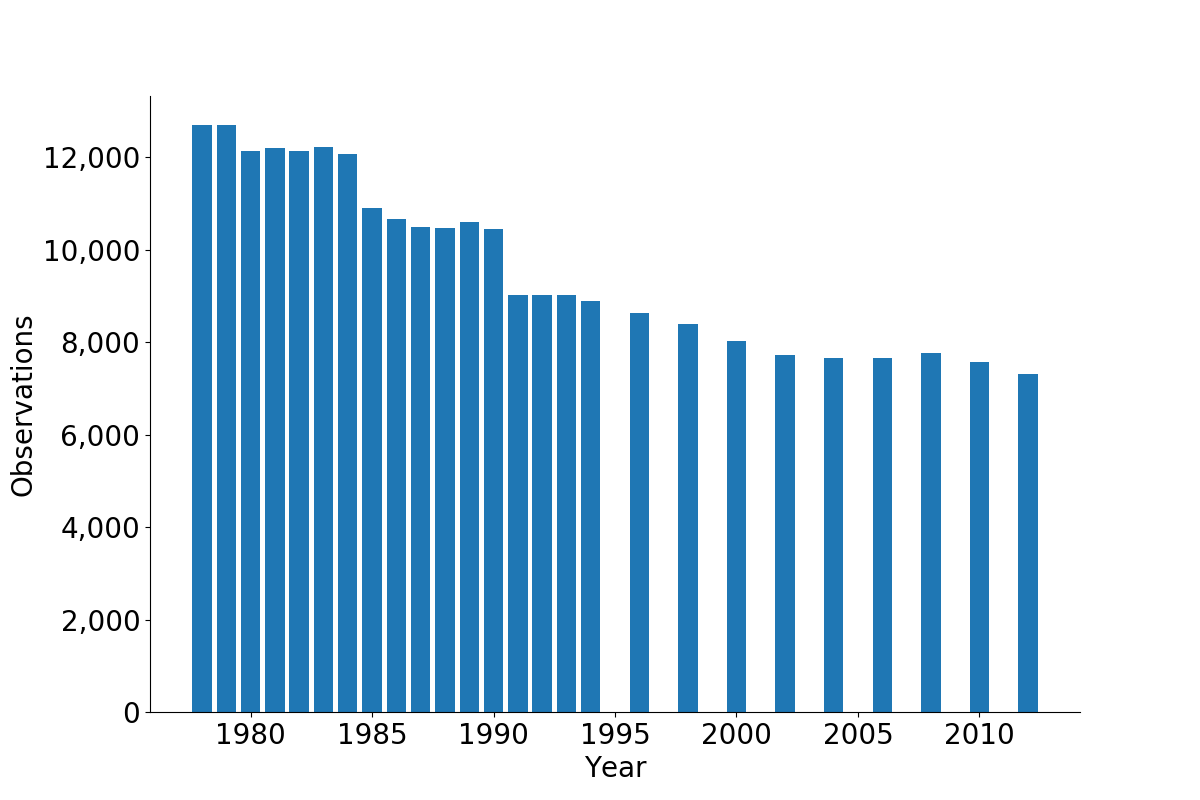
\includegraphics{fig-dataset-basic-observations}}
\end{figure}

\begin{figure}[htp]\centering
\caption{Number of Observations}
\scalebox{0.35}{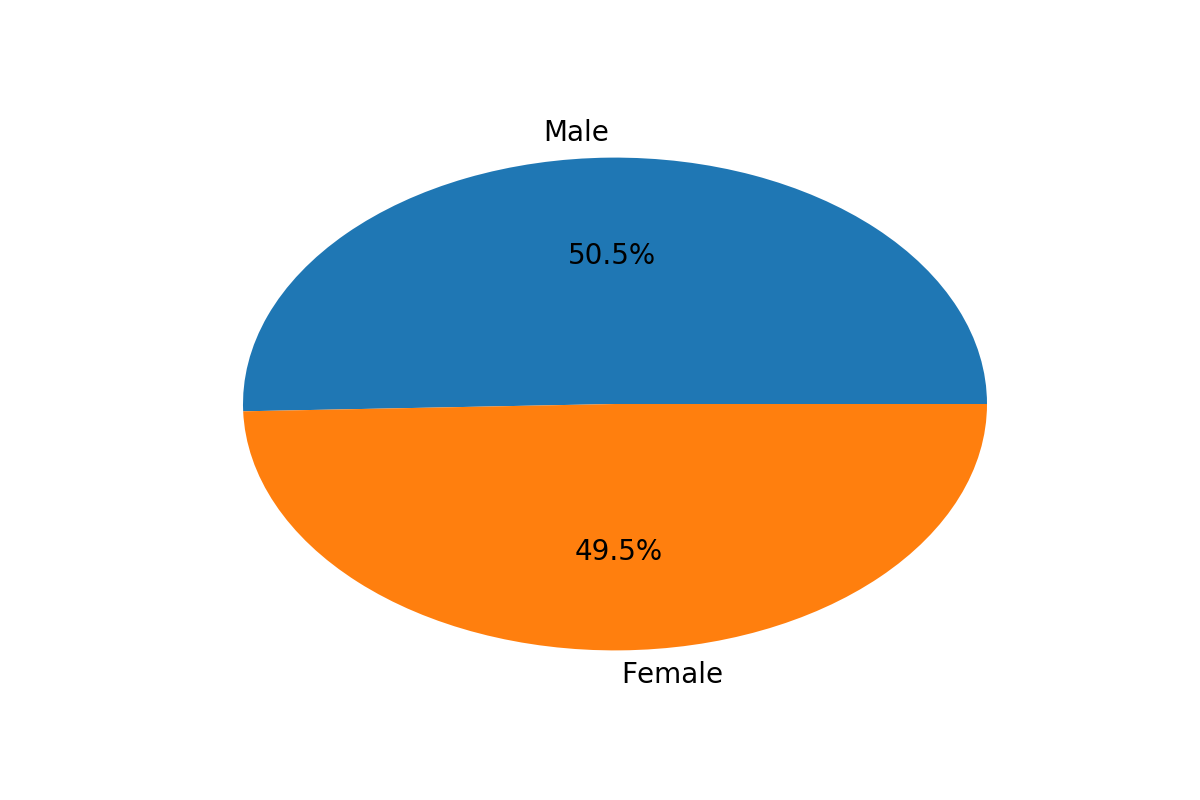
\includegraphics{fig-dataset-basic-gender}}
\end{figure}

\begin{figure}[htp]\centering
\caption{Number of Observations}
\scalebox{0.35}{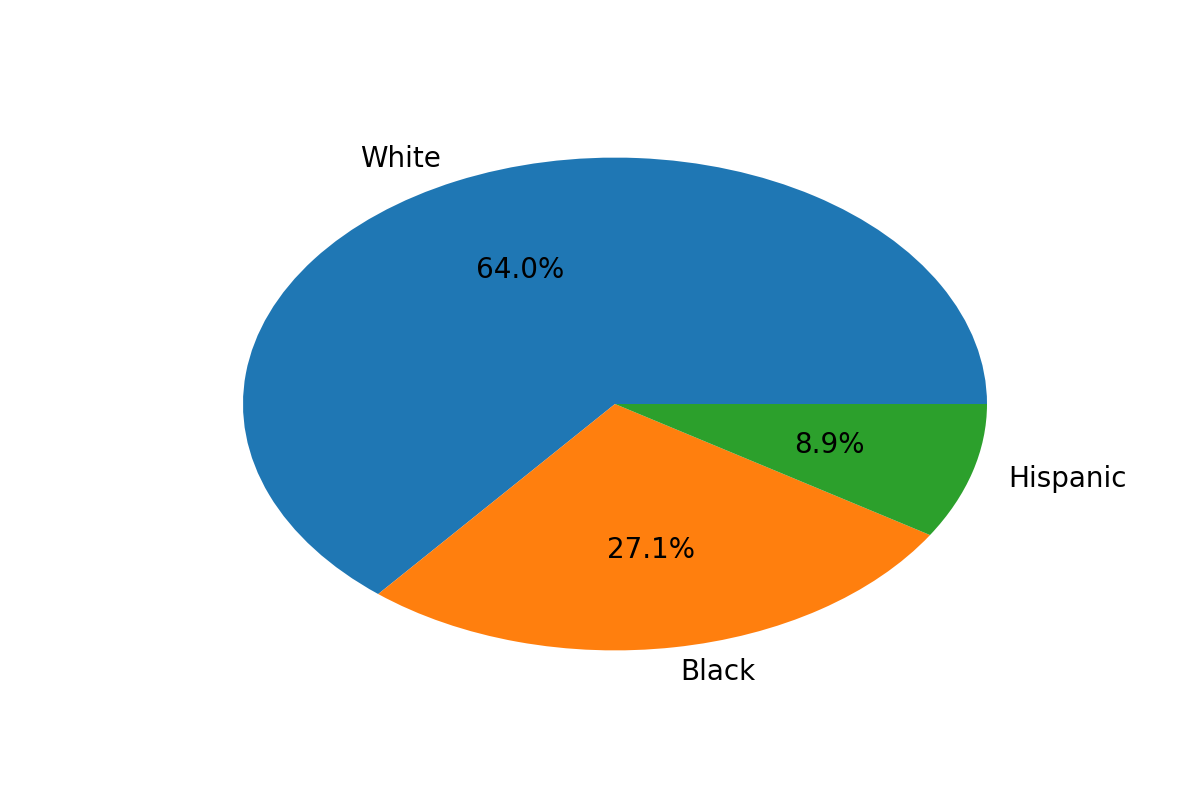
\includegraphics{fig-dataset-basic-race}}
\end{figure}

\begin{figure}[htp]\centering
\caption{Number of Observations}
\scalebox{0.35}{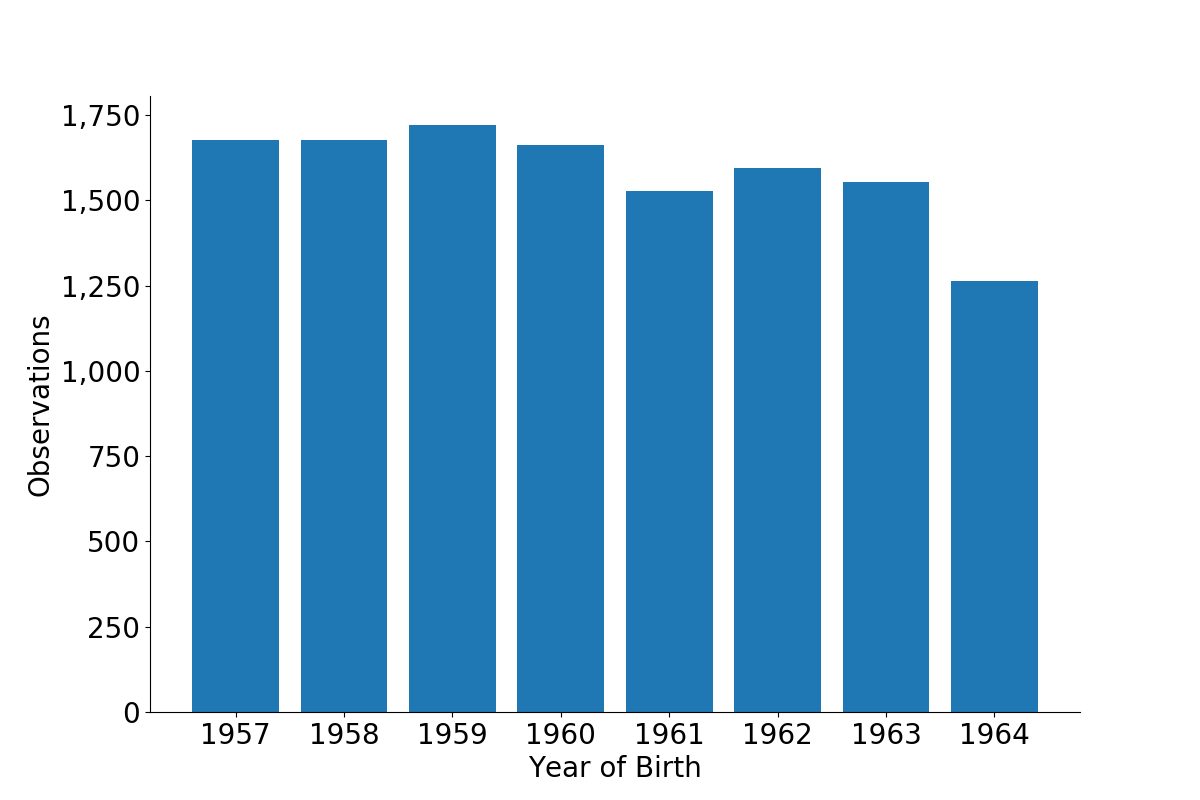
\includegraphics{fig-dataset-basic-birth}}
\end{figure}

%-------------------------------------------------------------------------------
\FloatBarrier\section{Cognitive Skills}
%-------------------------------------------------------------------------------
\begin{figure}[htp]\centering
\caption{ASVAB Arithmetic Reasoning}
\scalebox{0.35}{\includegraphics{fig-human-capital-cognitive-arithmetic-reasoning}}
\end{figure}

\begin{figure}[htp]\centering
\caption{ASVAB Word Knowledge}
\scalebox{0.35}{\includegraphics{fig-human-capital-cognitive-word-knowledge}}
\end{figure}

\begin{figure}[htp]\centering
\caption{ASVAB Paragraph Comprehension}
\scalebox{0.35}{\includegraphics{fig-human-capital-cognitive-paragraph-comprehension}}
\end{figure}

\begin{figure}[htp]\centering
\caption{ASVAB Numerical Operations}
\scalebox{0.35}{\includegraphics{fig-human-capital-cognitive-numerical-operations}}
\end{figure}

\begin{figure}[htp]\centering
\caption{AFQT Score}
\scalebox{0.35}{\includegraphics{fig-human-capital-cognitive-afqt}}
\end{figure}

\begin{figure}[htp]\centering
\caption{AFQT Score by race}
\scalebox{0.35}{\includegraphics{fig-human-capital-cognitive-race}}
\end{figure}
%-------------------------------------------------------------------------------
\FloatBarrier\section{Human Capital Basics}
%-------------------------------------------------------------------------------
The following graphs show the heatmap for the quartiles of selected skill measures and hourly local wages at age 35.

\begin{figure}[htp]\centering
\caption{AFQT Scores}
\scalebox{0.35}{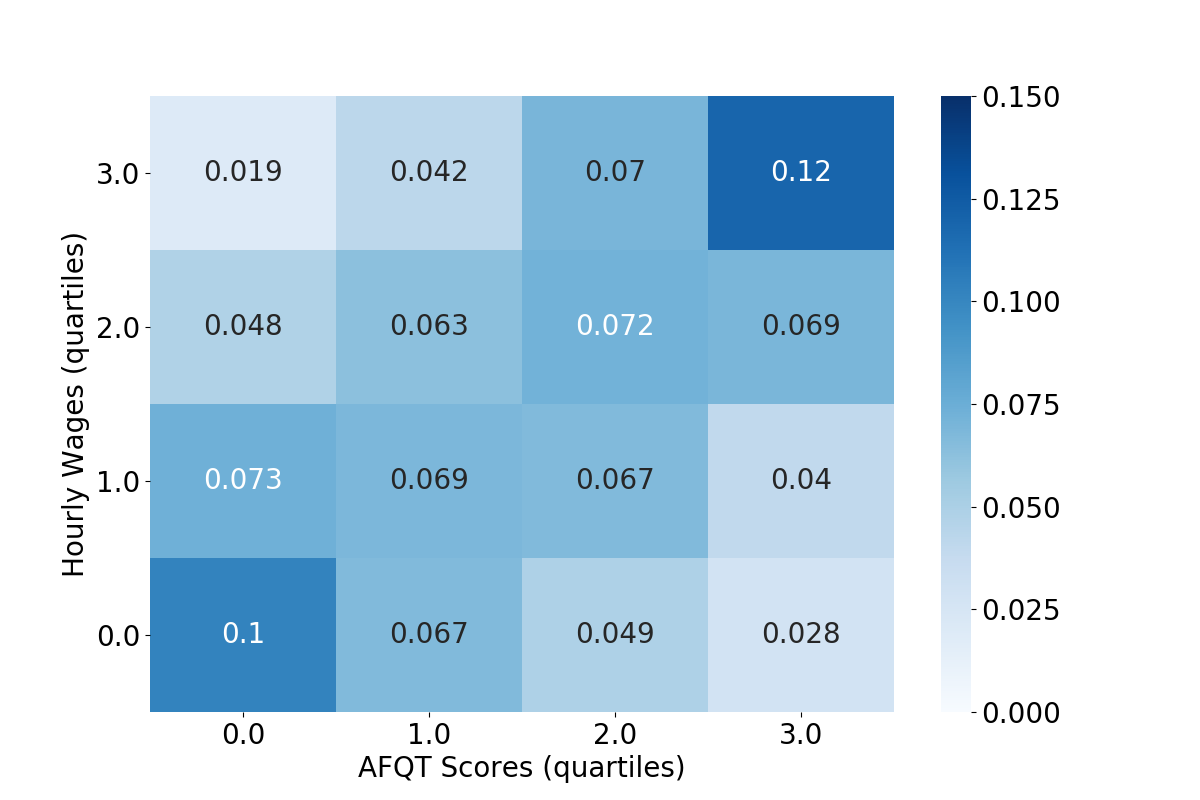
\includegraphics{fig-human-capital-basic-afqt}}
\end{figure}

\begin{figure}[htp]\centering
\caption{Rosenberg Scores}
\scalebox{0.35}{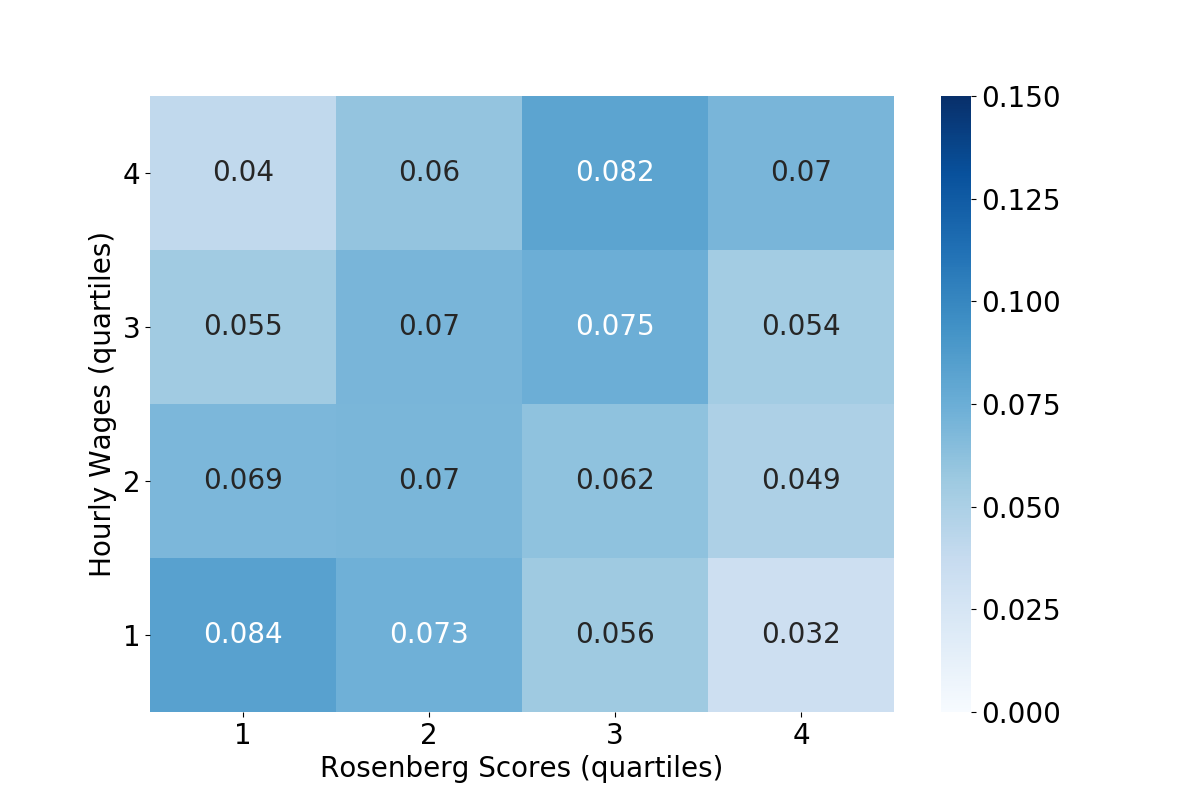
\includegraphics{fig-human-capital-basic-rosenberg}}
\end{figure}

\begin{figure}[htp]\centering
\caption{Rotter Scores}
\scalebox{0.35}{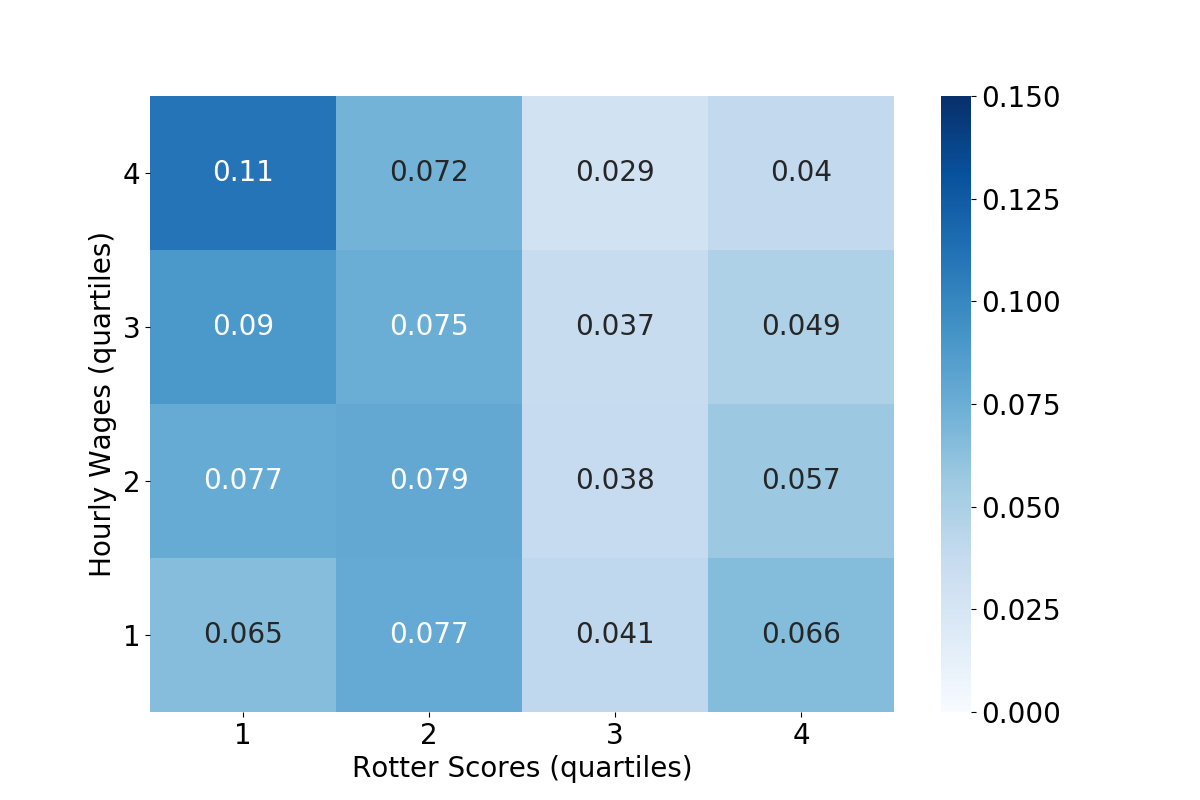
\includegraphics{fig-human-capital-basic-rotter}}
\end{figure}

%-------------------------------------------------------------------------------
\FloatBarrier\section{Intergenerational Transmission}
%-------------------------------------------------------------------------------
\begin{figure}[htp]\centering
\caption{Mother's Education}
\scalebox{0.35}{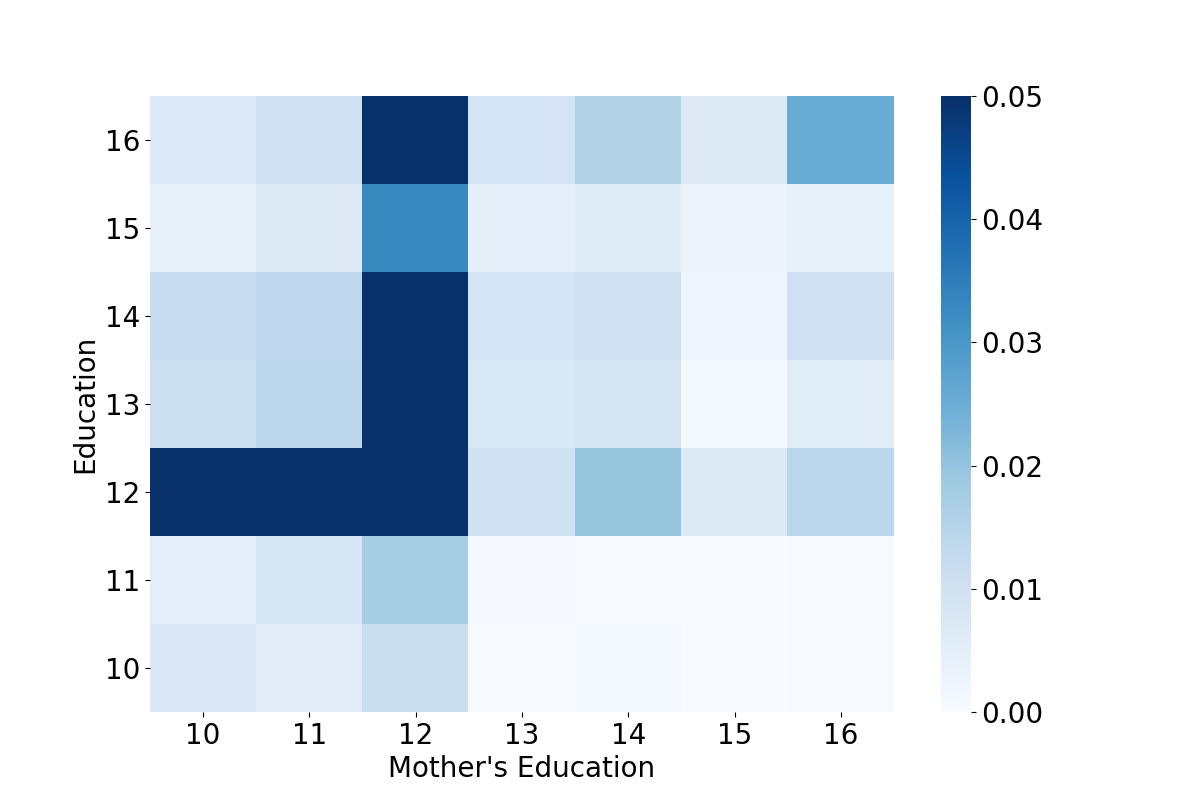
\includegraphics{fig-human-capital-intergenerational-mother}}
\end{figure}

\begin{figure}[htp]\centering
\caption{Father's Education}
\scalebox{0.35}{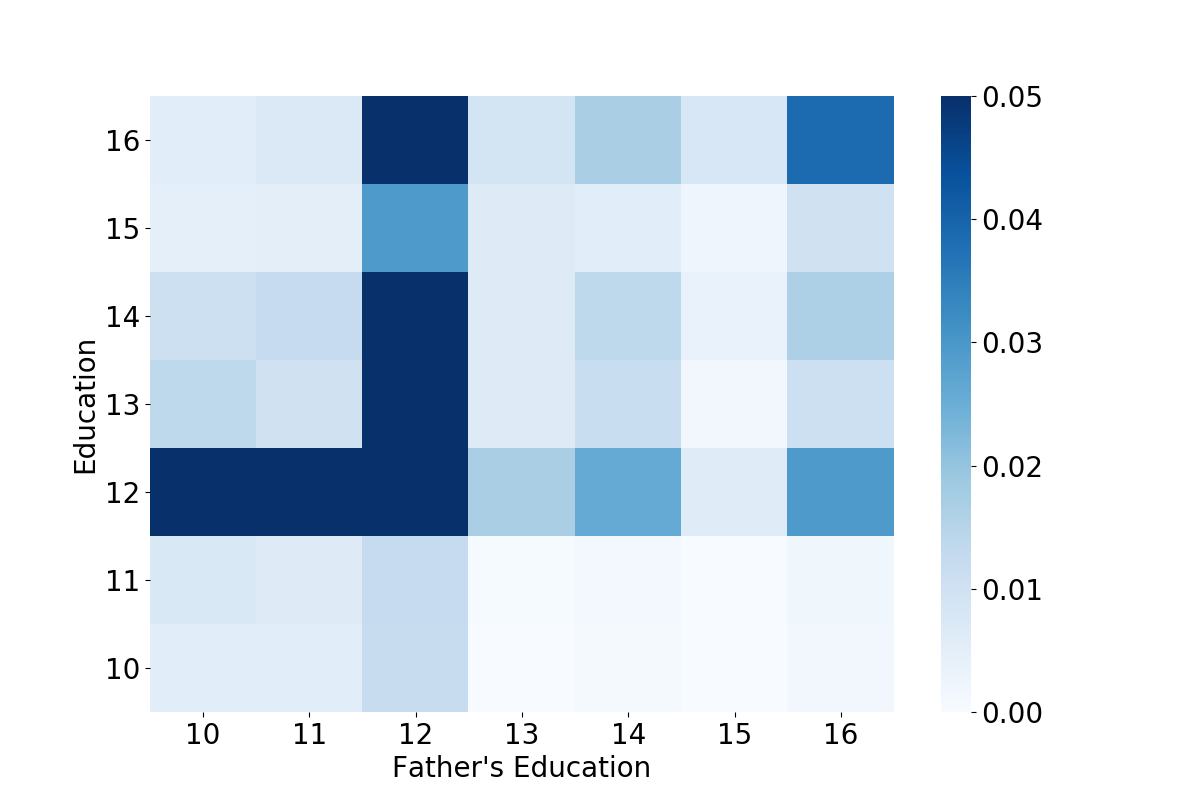
\includegraphics{fig-human-capital-intergenerational-father}}
\end{figure}

%-------------------------------------------------------------------------------
%-------------------------------------------------------------------------------
\FloatBarrier\section{Future improvements}

\begin{itemize}
\item Replace the figures from \citet{Spence.1973} with own creations.
\end{itemize}
